% !TEX root = ../../prj4projektdokumentation.tex
% SKAL STÅ I TOPPEN AF ALLE FILER FOR AT MASTER-filen KOMPILERES 

\section{Brugergrænseflade}
Brugergrænsefladerne der ses på figur \ref{fig:HMIAutomatikMode} og \ref{fig:HMIManuelMode} er udkast designet tidligt i processen før noget funktionalitet blev udviklet. Det er altså dem der er blevet brugt som udgangspunkt for det videre design. Det endelige design af brugergrænsefladerne kan ses i afsnit \ref{sec:HMI} Brugergrænseflade under Design.

\subsection{Automatisk mode}
\begin{figure}[H] % (alternativt [H])
	\centering
	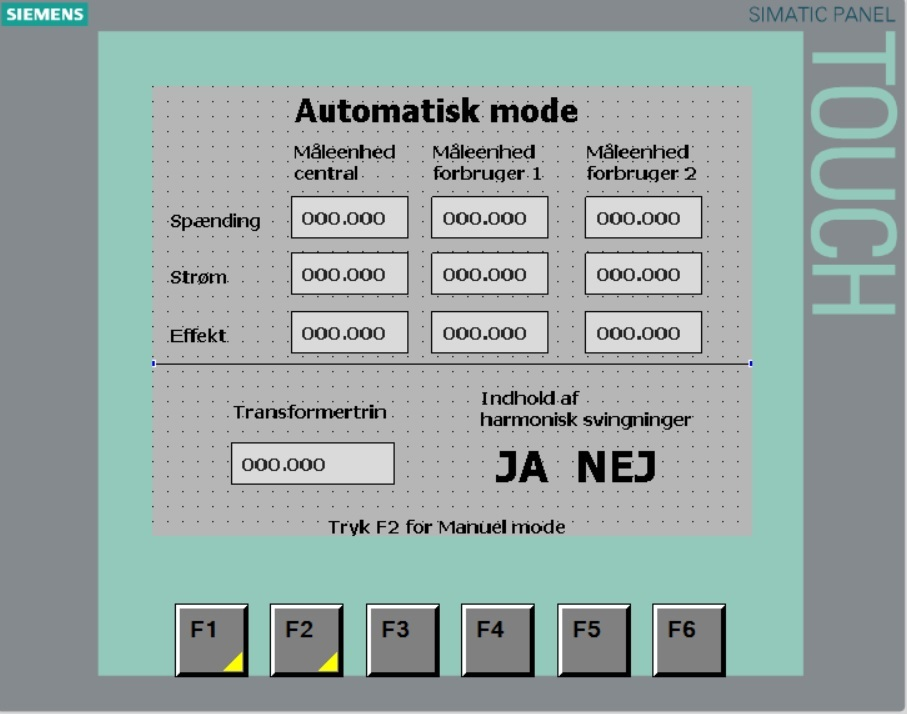
\includegraphics[width=0.9\textwidth]{Figure/HMIAutomatiskMode}
	\caption{HMI Automatisk mode}
	\label{fig:HMIAutomatikMode}
\end{figure}


\subsection{Manuel mode}
\begin{figure}[H] % (alternativt [H])
	\centering
	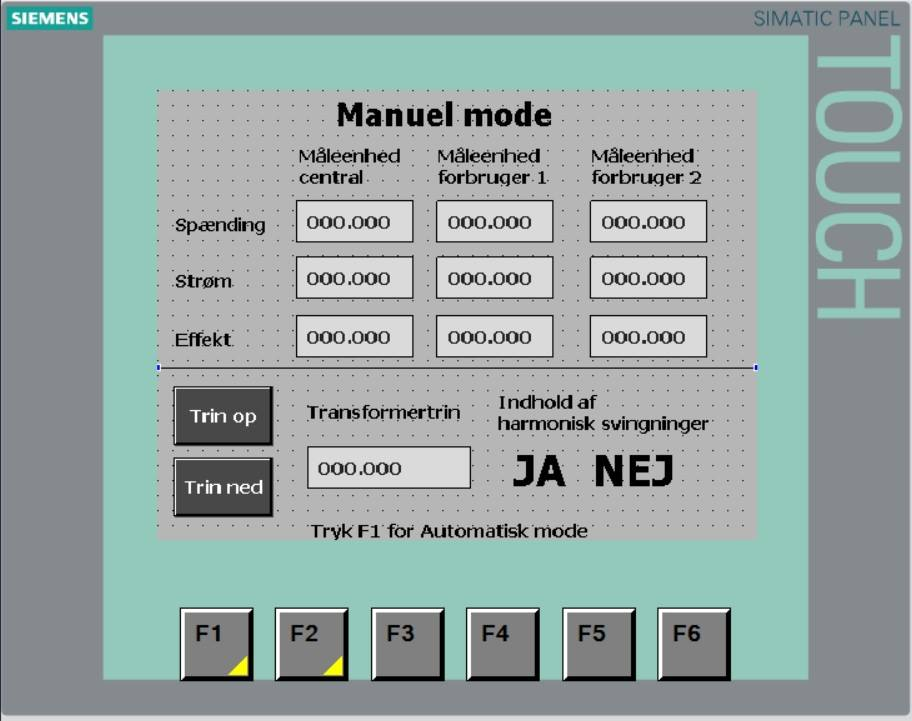
\includegraphics[width=0.9\textwidth]{Figure/HMIManuelMode}
	\caption{HMI Manuel mode}
	\label{fig:HMIManuelMode}
\end{figure}